\chapter{Proposed Solution}
\label{chap:solution}

\myLettrine{J}{ustifications} for usage of \gls{ccm} and \gls{dcm} are varied and each come with their trade-offs, however, given the inherent system properties and behaviour of \gls{dcm}, this makes it more suitable for current control in \gls{dc}-\gls{ac} systems as long as proper targets are set.
In this chapter, I will explain both the control algorithm, and showcase an ideal system's response using Simulink.

\section{Control of the H-bridge Converter in DCM}
\label{sec:dcmctrl}

\gls{dcm} leads to a nonlinear behaviour of the \gls{dc}-\gls{ac} converter which makes its control more difficult.
Although there are many control algorithms specific to nonlinear processes, their complexity restricts feasible implementations on microcontrollers.
To circumvent this limitation, the control method proposed is based around linearizing the converter operation and to use the classic \gls{pi} algorithm.
The source of the nonlinear behavior of the \gls{dc}-\gls{ac} converter is given by the value of the average current through the inductor which is:
\begin{equation}
    \label{eq:medindcur}
    (I_L)_{med} =  \left\{
        \begin{aligned}
            \frac{V_S}{2 \cdot L \cdot T_o} \cdot \frac{V_S - U_C}{U_C} \cdot T_h^2,   I_o > 0 \\
            \frac{V_S}{2 \cdot L \cdot T_o} \cdot \frac{U_C}{V_S - U_C} \cdot T_l^2,   I_o < 0 \\
        \end{aligned}
    \right.
\end{equation}

It can be noted that the current value depends on the operation point of the converter (represented by capacitor voltage $U_C$) and the square of the command variable ($T_h$ or $T_l$).
The main idea to obtain a linear operation of the converter is to make the inductor current depend only on the control variable and its dependence to be linear.
As a result, the assembly that is consisting of the half-bridge and the inductor will behave as an ideal controlled current source.

The solution for linearization is to measure the capacitor voltage $U_C$ and compute the time values $T_h$ and $T_l$ as following:
\begin{equation}
    \left\{
        \begin{aligned}
            \label{eq:timecalc}
            T_h = T_o \cdot \sqrt{\frac{U_C}{V_S - U_C} \cdot q^+},   I_o > 0 \\
            T_l = T_o \cdot \sqrt{\frac{V_S - U_C}{U_C} \cdot q^-},   I_o < 0
        \end{aligned}
    \right.
\end{equation}
where $q^+$ is the new command variable for generating a positive output current and $q^-$ is the new command variable for generating negative current.
If the output current is positive, the command value will be applied on $q^+$ and the high-side transistor will be switched on for the time interval equal to:
\begin{equation}
    T_h = T_o \cdot \sqrt{\frac{U_C}{V_S - U_C} \cdot q^+}
\end{equation}
In this case, the average value of the inductor current is:
\begin{equation}
    \begin{split}
        (I_L)_{med} &= \frac{V_S}{2 \cdot L \cdot T_o} \cdot \frac{V_S - U_C}{U_C} \cdot T_h^2 \\
        &= \frac{V_S}{2 \cdot L \cdot T_o} \cdot \frac{V_S - U_C}{U_C} \cdot \left(T_o \cdot \sqrt{\frac{U_C}{V_S - U_C} \cdot q^+}\right)^2 \\
        &= \frac{V_S}{2 \cdot L \cdot T_o} \cdot \frac{V_S - U_C}{U_C} \cdot T_o^2 \cdot \frac{U_C}{V_S - U_C} \cdot q^+ \\
        &= \frac{V_S \cdot T_o}{2 \cdot L} \cdot q^+
    \end{split}
\end{equation}

It can be noted that the half-bridge and inductor assembly generates an output current that depends linearly on the command variable $q^+$ and is no longer influenced by the capacitor voltage $U_C$ exactly like a controlled current source.

Similarly, if the output current is negative, the command value will be applied on $q^-$ and the low-side transistor will be switched on for the time interval equal to:
\begin{equation}
    T_l = T_o \cdot \sqrt{\frac{V_S - U_C}{U_C} \cdot q^-}
\end{equation}
and the average value of the inductor current will be:
\begin{equation}
    \begin{split}
        (I_L)_{med} &= \frac{V_S}{2 \cdot L \cdot T_o} \cdot \frac{U_C}{V_S - U_C} \cdot T_l^2 \\
        &= \frac{V_S}{2 \cdot L \cdot T_o} \cdot \frac{U_C}{V_S - U_C} \cdot \left(T_o \cdot \sqrt{\frac{V_S - U_C}{U_C} \cdot q^-}\right)^2 \\
        &= \frac{V_S}{2 \cdot L \cdot T_o} \cdot \frac{U_C}{V_S - U_C} \cdot T_o^2 \cdot \frac{V_S - U_C}{U_C} \cdot q^- \\
        &= \frac{V_S \cdot T_o}{2 \cdot L} \cdot q^-
    \end{split}
\end{equation}
that also corresponds to a linear controlled current source.

In microgrid systems, the load of the \gls{dc}-\gls{ac} converter should have low internal resistance for increased conversion efficiency.
As such, an additional inductor must be placed between the filter capacitor and the output connected to the grid.
\begin{figure}[!ht]
    \begin{center}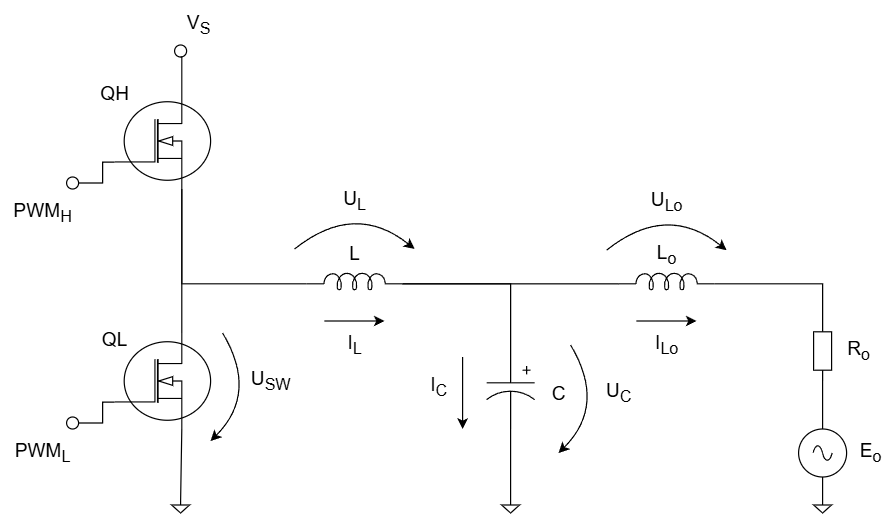
\includegraphics[width=\singlefigure]{\pics/models/halfmodel}\end{center}
    \caption{Half-bridge model connected to a load}
    \label{fig:halfmodel}
\end{figure}
The equivalent model of the whole system is the following:
\begin{figure}[!ht]
    \begin{center}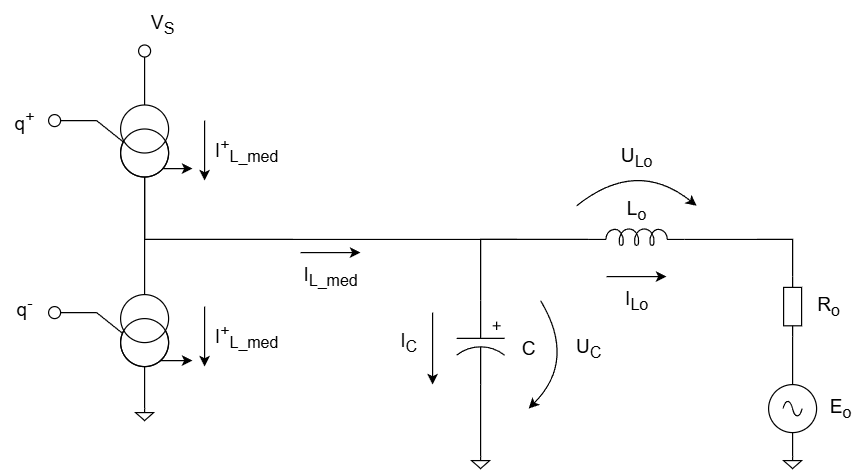
\includegraphics[width=\singlefigure]{\pics/models/halfsimplified}\end{center}
    \caption{Half-bridge simplified model connected to a load}
    \label{fig:halfsimplified}
\end{figure}
The output current value is:
\begin{equation}
    \begin{split}
        I_o(s) &= \frac{1}{L_o \cdot C \cdot s^2 + R_o \cdot C \cdot s + 1}(I_L)_{med}(s) \\
        &= \frac{1}{L_o \cdot C \cdot s^2 + R_o \cdot C \cdot s + 1} \cdot \left[(I_L^+)_{med}(s) - (I_L^-)_{med}(s)\right] \\
        &= \frac{1}{L_o \cdot C \cdot s^2 + R_o \cdot C \cdot s + 1} \cdot \frac{V_S \cdot T_o}{2 \cdot L} \cdot \left[q^+(s) - q^-(s)\right] \\
    \end{split}
\end{equation}
that corresponds to an equivalent second-order system:
\begin{equation}
    I_o(s) = K_C \cdot \frac{\omega^2}{s^2 + 2 \cdot \zeta \omega + \omega^2} \cdot \left[q^+(s) - q^-(s)\right]
\end{equation}
where:
\begin{align*}
    K_C = \frac{V_S \cdot T_o}{2 \cdot L},  &&   \omega = \sqrt{\frac{1}{L_o \cdot C}},  &&   \zeta = \frac{R_o}{2} \cdot \sqrt{\frac{C}{L_o}}
\end{align*}

The low value of the internal resistance $R_o$ leads to a small value of the damping factor $\zeta$.
Therefore, the output current will have a strongly oscillating response to variations in the command.
Utilizing passive electronics for damping this negative effect is not an ideal solution because they generate additional energy losses.
A better approach is to emulate the effect of the passive damping circuits inside the control algorithm, as shown in \figref{fig:outfiltr}.
\begin{figure}[!ht]
    \begin{center}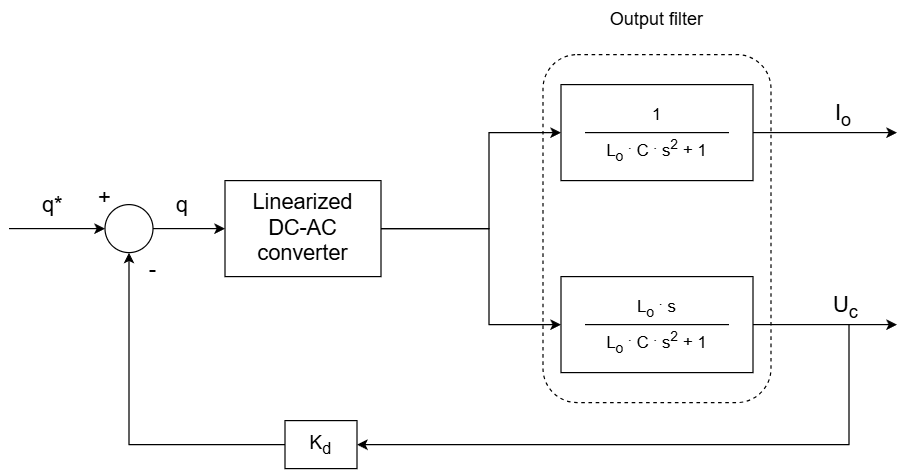
\includegraphics[width=\singlefigure]{\pics/models/controlsch}\end{center}
    \caption{Proposed control scheme for current control}
    \label{fig:outfiltr}
\end{figure}
For simplicity, the internal resistance $R_o$ is considered zero which is consistent with the real scenario where this value is insignificant.
The new command variable for the converter ($q^*$) and its feedback effect is:
\begin{equation}
    \begin{split}
        \label{eq:newcmd}
        q &= q^* - K_d \cdot U_C = q^* - K_d \cdot \frac{L_o \cdot s}{L_o \cdot C \cdot s^2 + 1} \cdot (I_L)_{med} \\
        &= q^* - K_d \cdot \frac{L_o \cdot s}{L_o \cdot C \cdot s^2 + 1} \cdot \frac{V_S}{2 \cdot L \cdot T_o} \cdot q
    \end{split}
\end{equation}
The value of the feedback coefficient is chosen according to the desired damping factor $\zeta^*$ using the following equation:
\begin{equation}
    K_d = 2 \cdot \zeta^* \cdot \frac{2 \cdot L}{V_S \cdot T_o} \cdot \sqrt{\frac{C}{L_o}}
\end{equation}
Substituting this value into \eqref{eq:newcmd}, the command can be written as:
\begin{equation}
    \begin{split}
        q &= q^* - 2 \cdot \zeta^* \cdot \frac{2 \cdot L}{V_S \cdot T_o} \cdot \sqrt{\frac{C}{L_o}} \cdot \frac{L_o \cdot s}{L_o \cdot C \cdot s^2 + 1} \cdot \frac{V_S}{2 \cdot L \cdot T_o} \cdot q \\
        &= q^* - 2 \cdot \zeta^* \cdot \sqrt{\frac{C}{L_o}} \cdot \frac{L_o \cdot s}{L_o \cdot C \cdot s^2 + 1} \cdot q \\
        &= q^* - \frac{2 \cdot \zeta^* \cdot \sqrt{L_o \cdot C} \cdot s}{L_o \cdot C \cdot s^2 + 1} \cdot q
    \end{split}
\end{equation}
which turns into:
\begin{equation}
    q = q^* \cdot \frac{L_o \cdot C \cdot s^2 + 1}{L_o \cdot C \cdot s^2 + 2 \cdot \zeta^* \cdot \sqrt{L_o \cdot C} \cdot s + 1}
\end{equation}
The output current value becomes:
\begin{equation}
    \label{eq:outputcurrent}
    \begin{split}
        I_o &= \frac{1}{L_o \cdot C \cdot s^2 + 1} \cdot q \\
        &= \frac{1}{L_o \cdot C \cdot s^2 + 1} \cdot q^* \cdot \frac{L_o \cdot C \cdot s^2 + 1}{L_o \cdot C \cdot s^2 + 2 \cdot \zeta^* \cdot \sqrt{L_o \cdot C} \cdot s + 1} \\
        &= q^* \cdot \frac{1}{L_o \cdot C \cdot s^2 + 2 \cdot \zeta^* \cdot \sqrt{L_o \cdot C} \cdot s + 1} \\
        &= \frac{\frac{1}{L_o \cdot C}}{s^2 + 2 \cdot \zeta^* \cdot \sqrt{\frac{1}{L_o \cdot C}} \cdot s + \frac{1}{L_o \cdot C}} \cdot q^*
    \end{split}
\end{equation}
that corresponds to a second-order system with the following parameters:
\begin{align*}
    K = 1,      &&  \omega = \sqrt{\frac{1}{L_o \cdot C}},      &&  \zeta = \zeta^*
\end{align*}

So far, the proposition of the linear control of the circuit has been demonstrated using a half-bridge circuit as reference, however this is still valid for an \gls{H-bridge}, as the construction in itself is mirrored on the opposite side of the load.
To be noted that under \tabref{tab:switchfunc}, the valid states for current conduction are only states 1 and 2, thus $S_4$ and $S_2$ have inverted functionalities, with the low-side transistor $S_4$ having the same switching signals as high-side transistor $S_1$.
This would in turn mean that the same energy that is injected into the system is also ejected on the other side of the circuit.
Knowing this, it would mean that in order to prove that the system is equivalent to the half-bridge model, the source voltage injected is the sum of the two voltages across both filter capacitors ($V_S = U_{C1} + U_{C2}$).
\begin{equation}
    \label{eq:hbridgeproof}
    I_o =  \left\{
        \begin{aligned}
            \frac{V_S}{2 \cdot L \cdot T_o} \cdot \frac{V_S - U_{C1}}{U_{C1}} \cdot T_{h1}^2, I_o \rightarrow output \ current\\
            \frac{V_S}{2 \cdot L \cdot T_o} \cdot \frac{U_{C2}}{V_S - U_{C2}} \cdot T_{l2}^2, I_o \rightarrow input \ current 
        \end{aligned}
    \right.
\end{equation}
Equation \eqref{eq:hbridgeproof} is adapted from equation \eqref{eq:medindcur}, where the only varying terms are the voltages across each capacitor.
Since the input current is the same as the output current, and based on switching state 1 and 2 which results that $T_{h1} = T_{l2}$, the relation can be written as:
\begin{equation}
    \begin{split}
        \frac{V_S}{2 \cdot L \cdot T_o} \cdot \frac{V_S - U_{C1}}{U_{C1}} \cdot T_{h1}^2 &= \frac{V_S}{2 \cdot L \cdot T_o} \cdot \frac{U_{C2}}{V_S - U_{C2}} \cdot T_{l2}^2 \\
        \frac{V_S - U_{C1}}{U_{C1}} &= \frac{U_{C2}}{V_S - U_{C2}} \\
        U_{C1} \cdot U_{C2} &= (V_S - U_{C1})(V_S - U_{C2}) \\
        U_{C1} \cdot U_{C2} &= V_S^2 - V_S U_{C1} - V_S U_{C2} + U_{C1} U_{C2} \\
        V_S^2 &= V_S(U_{C1} + U_{C2}) \\
        V_S &= U_{C1} + U_{C2}
    \end{split}
\end{equation}

To conclude this section, the steps that describe the algorithm for a linear operation of the \gls{dc}-\gls{ac} converter in \gls{dcm} are:
\begin{enumerate}
    \item Compute $q = q^* - K_d \cdot U_C = q - 2 \cdot \zeta^* \cdot \frac{2 \cdot L}{V_S \cdot T_o} \cdot \sqrt{\frac{C}{L_o}} \cdot U_C$;
    \item If $q > 0$, apply the \gls{pwm} signals with the duration $T_h = T_o \cdot \sqrt{\frac{U_C}{V_S - U_C} \cdot q}$ on the high-side transistor, else apply \gls{pwm} signals with the duration $T_l = T_o \cdot \sqrt{\frac{V_S - U_C}{U_C} \cdot q}$ on the low-side transistor.
\end{enumerate}

\section{Model Recreation in Simulink}
\label{sec:simrec}

\begin{table}[ht!]
\begin{center}
\begin{tabular}{|c|c|c|c|}
\hline
System parameter&Unit of measurement&Value&Description\\ \hline
$V_S$&$V$&$24$&Input source DC voltage\\ \hline
$E_o$&$V$&$12$&Output source peak AC voltage\\ \hline
$C_1, C_2$&$\mu F$&$100$&Filter capacitance\\ \hline
$L_1, L_2$&$\mu H$&$12$&Source filter inductance\\ \hline
$L_o$&$\mu H$&$108$&Output current filter inductance\\ \hline
$T_s$&$ns$&$20$&Simulation sample time\\ \hline
$F_o$&$KHz$&$50$&PWM base frequency\\ \hline
$T_o$&$\mu s$&$20$&PWM time period\\ \hline
ESR&$m\Omega$&$1$&Equivalent Series Resistance \\
&&&of the passive components\\ \hline
\end{tabular}
\end{center}
\caption{Values used in the simulated model}
\label{tab:simvals}
\end{table}
While theoretical context and the proposed solution have been presented, there's no guarantee these are valid unless testing through simulation is achieved.
This is done with some considerations in mind, such as power conversion target values, component tolerances, and simulation program limitations.
Regardless of these, it should be noted that results are affected how simulation parameters are set up and how the simulation engine works, which will be detailed later in this chapter.
These values are described in \tabref{tab:simvals}, and the parameter names correspond to variable names used in the Simulink model.

Target voltages can be chosen based on experimental expectations, however values like filter capacitance and inductance are chosen in order to cut out high band frequencies detrimental to the system's conversion, such as the residual \gls{pwm} switching or secondary harmonics of the output grid voltage.
Having all the base parameters set for this system, we can create the electrical model using Simulink and Simscape toolbox which can emulate the circuits needed for the plant and feedback loop.
\begin{figure}[!ht]
    \centering
    \makebox[0pt]{
        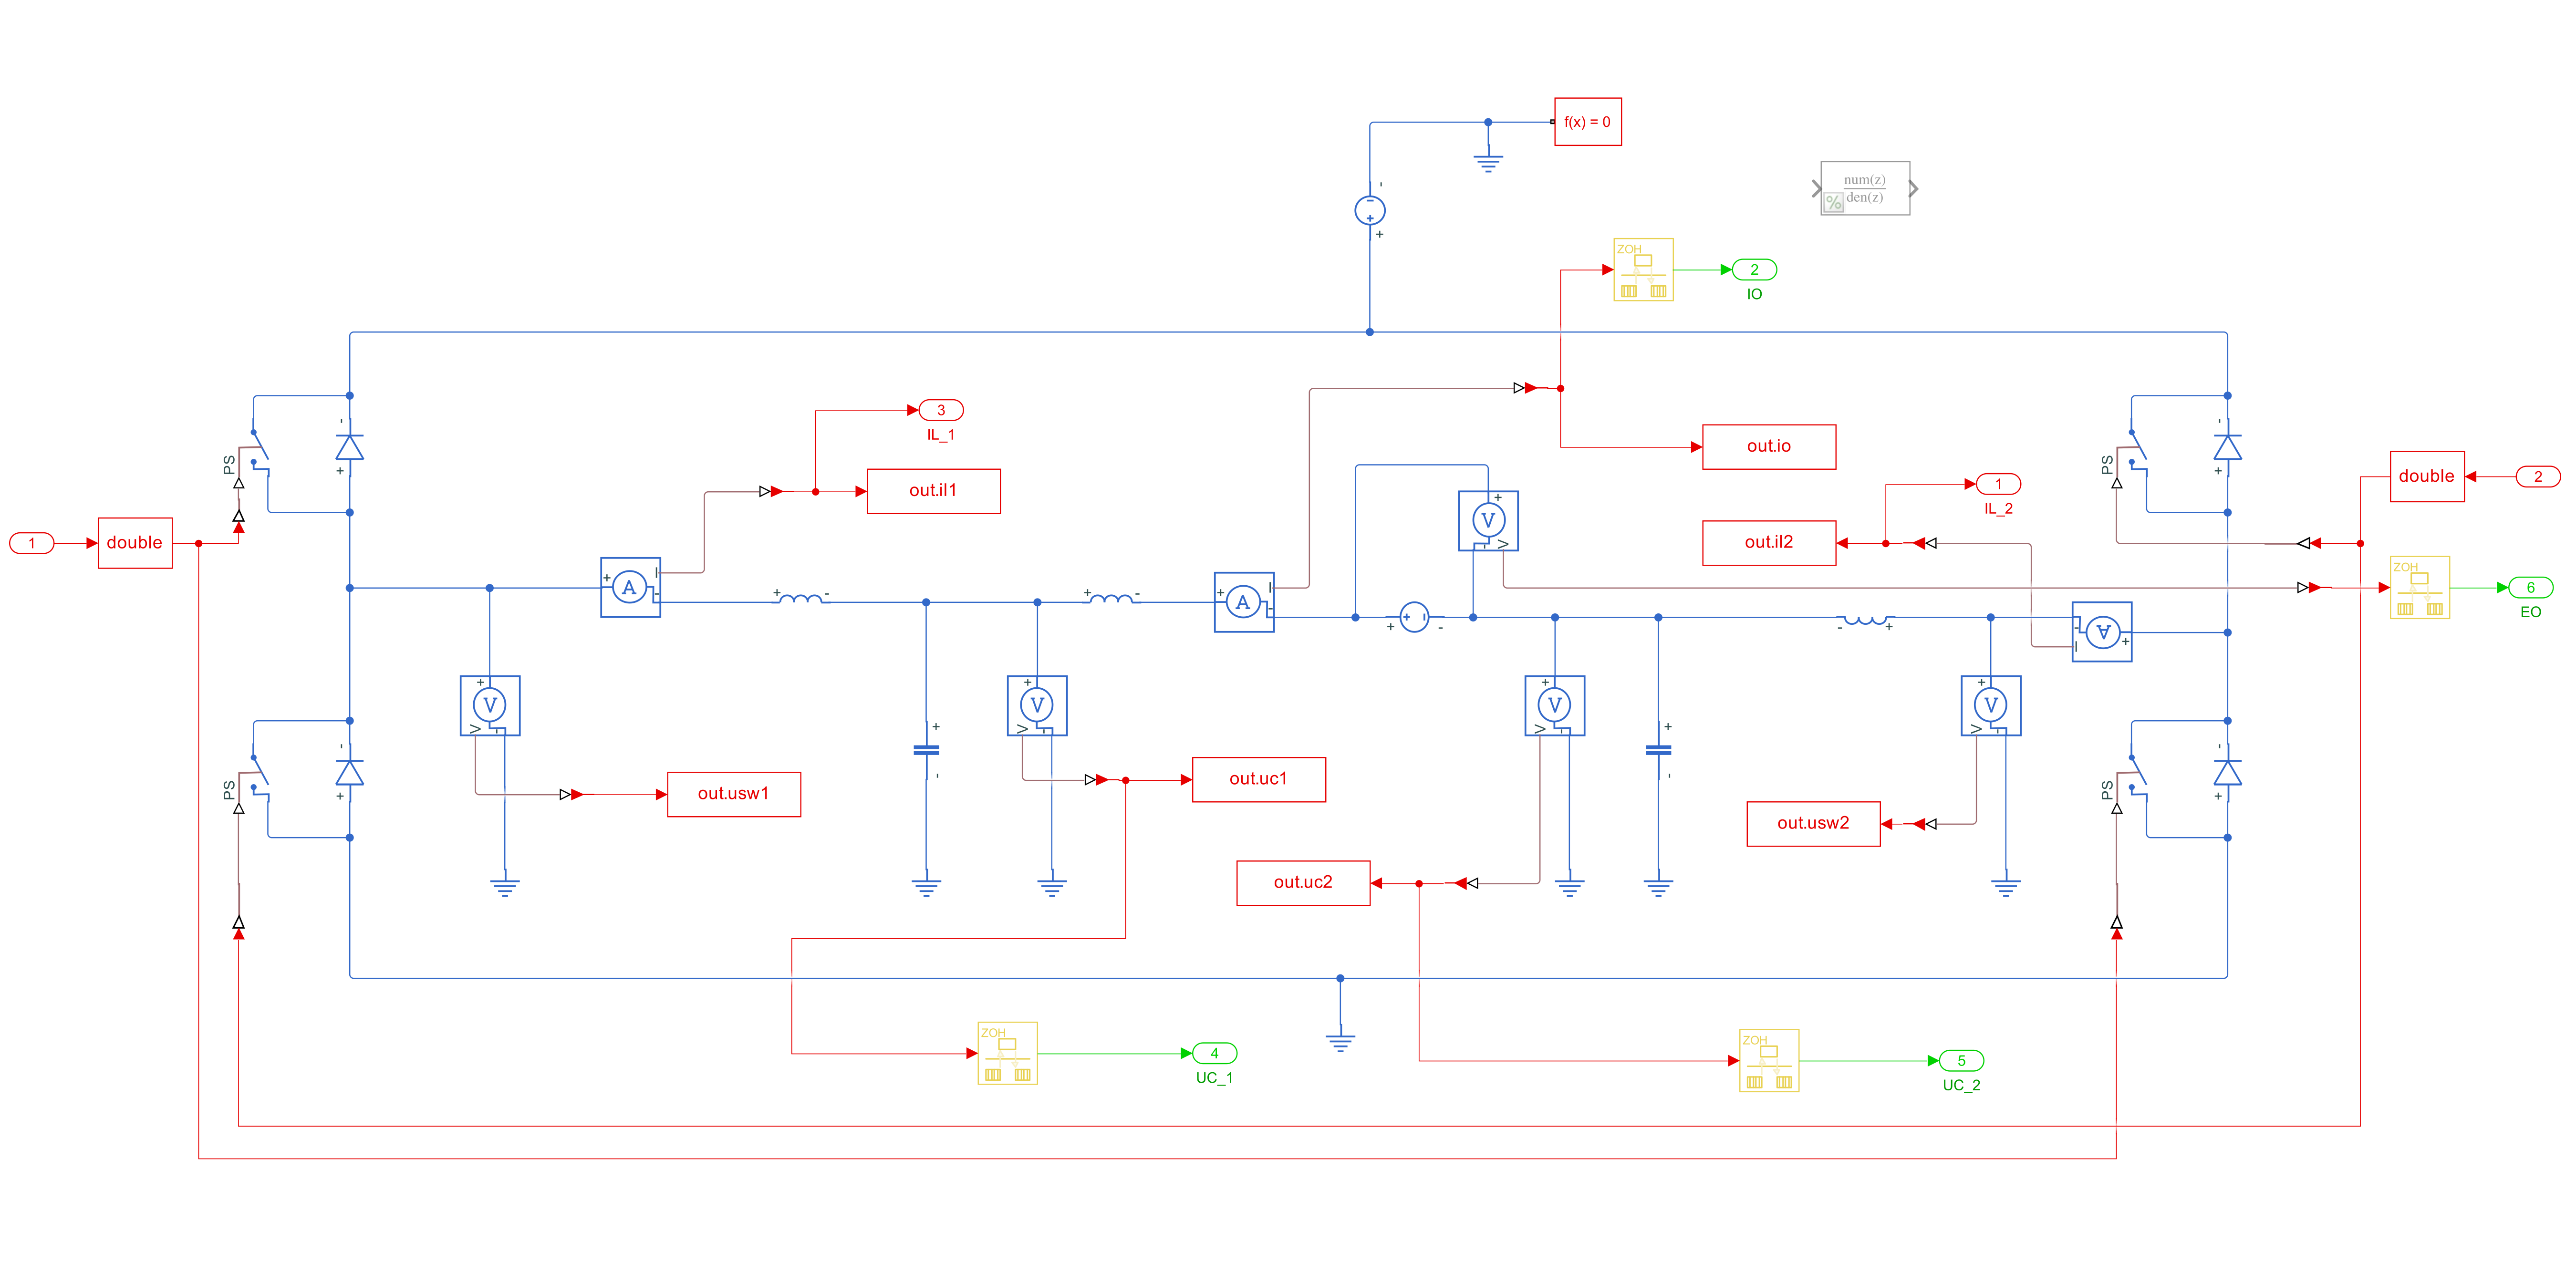
\includegraphics[width=0.95\paperwidth]{\pics/simulink/hbridge}
    }
    \caption{Simulink model of the H-bridge}
    \label{fig:simhbridge}
\end{figure}
Looking at \figref{fig:simhbridge}, MOSFETs have been emulated using ideal switches with a body diode oriented opposite to the direction of the voltage created by the input source.
Other passive components have low \gls{esr} as to not affect the study of the ideal model in any major way.
Currents and voltages have been measured across both output points and intermediate points at components to make sure that the system behaviour matches the theoretical model, and that the control feedback loop can be implemented.
As pointed by \figref{fig:outfiltr}, there's a need for the capacitor voltage in order to create the appropriate $K_d$ gain amplification term that is used for the linearized function of the system.
Since the final goal of the application is to regulate the output current of the converter, $I_o$ has to be measured each $T_o$ in order to compensate the command.

While the model's linearization has been demonstrated in the previous equations, in order to create a constant power source out of the described topology, a \gls{pi} controller has to be connected to the feedback loop in order to create a current with the value equal to the desired reference of the system.
The controller transfer function is defined as:
\begin{equation}
    \begin{split}
        H_r(s) &= P + I \frac{1}{s} \\
        &= \frac{I + Ps}{s} \\
        &= \frac{I\left(1 + \frac{P}{I}s\right)}{s}
    \end{split}
\end{equation}
Knowing that equation \eqref{eq:outputcurrent} describes the relation between the new command and output current, the transfer function of the open feedback is:
\begin{equation}
    \begin{split}
        \frac{I_o(s)}{q^*(s)} &= \frac{\frac{1}{L_o \cdot C}}{s^2 + 2 \cdot \zeta^* \cdot \sqrt{\frac{1}{L_o \cdot C}} \cdot s + \frac{1}{L_o \cdot C}},\ choosing \ \zeta^* = 1 \\
        H_p(s) &= \frac{1}{L_o \cdot C \cdot s^2 + 2 \sqrt{L_o \cdot C} \cdot s + 1} \\
        &= \frac{1}{(\sqrt{L_o \cdot C} \cdot s + 1)^2} \\
        &= \frac{K_p}{(Ts + 1)^2}
    \end{split}
\end{equation}
This is useful twofold, since this demonstrates that the system can be written as a first-order system with a double pole, meaning \gls{pi} control is achievable, and because in order to determine the transfer function of the controller, the closed feedback loop system is written as:
\begin{equation}
    \begin{split}
        H_o(s) &= \frac{H_r(s) H_p(s)}{1 + H_r(s) H_p(s)} \\
        &= \frac{\frac{I\left(1 + \frac{P}{I}s\right)}{s} \cdot \frac{K_p}{(Ts + 1)^2}}{ 1 + \frac{I\left(1 + \frac{P}{I}s\right)}{s} \cdot \frac{K_p}{(Ts + 1)^2}} \\
        \ if \ \frac{P}{I} = T \Rightarrow I = \frac{P}{T} \Rightarrow \\
        H_o(s) &= \frac{\frac{P}{T} \cdot \frac{1 + Ts}{s} \cdot \frac{K_p}{(T_s + 1)^2}}{1 + \frac{P}{Ts} \cdot \frac{K_p}{Ts + 1}} \\
        &= \frac{\frac{P K_p}{Ts (Ts + 1)}}{1 + \frac{P K_p}{Ts (Ts + 1)}} \\
        &= \frac{P K_p}{P K_p + Ts(Ts + 1)} \\
        &= \frac{P K_p}{T^2 s^2 + T s + P K_p} \\
        &= \frac{\frac{P K_p}{T^2}}{s^2 + \frac{1}{T}s + \frac{P K_p}{T^2}} \\
    \end{split}
\end{equation}
This form follows a second order transfer function, with natural frequency $\omega_n$ and system damping ratio $\zeta$ being described using proportional and process time constants $P$ and $T$:
\begin{align*}
    \omega_n = \frac{P K_p}{T^2}, && 2 \zeta \omega_n = \frac{1}{T}
\end{align*}
Using this, we can compute the values for \gls{pi} controller constants in this manner:
\begin{equation}
    \begin{split}
        2 \zeta \sqrt{\frac{P K_p}{T^2}} = \frac{1}{T} &\Rightarrow \frac{2 \zeta}{T} \sqrt{P K_p} = \frac{1}{T} \Rightarrow \\
        2 \zeta \sqrt{P K_p} = 1 &\Rightarrow \sqrt{P K_p} = \frac{1}{2 \zeta}; \\
        \ as \ \zeta = 1 \Rightarrow \sqrt{P K_p} = \frac{1}{2} &\Rightarrow P K_p = \frac{1}{4} \Rightarrow P = \frac{1}{4 K_p}
    \end{split}
\end{equation}
The $K_p$ term is the gain amplification term present in the transfer function of the plant, which is present if we simulate the step response of the open loop system.
For this, we first have to describe the entirety of the control system, which is presented in \figref{fig:discuinv}.
\begin{figure}[!ht]
    \centering
    \makebox[0pt]{
        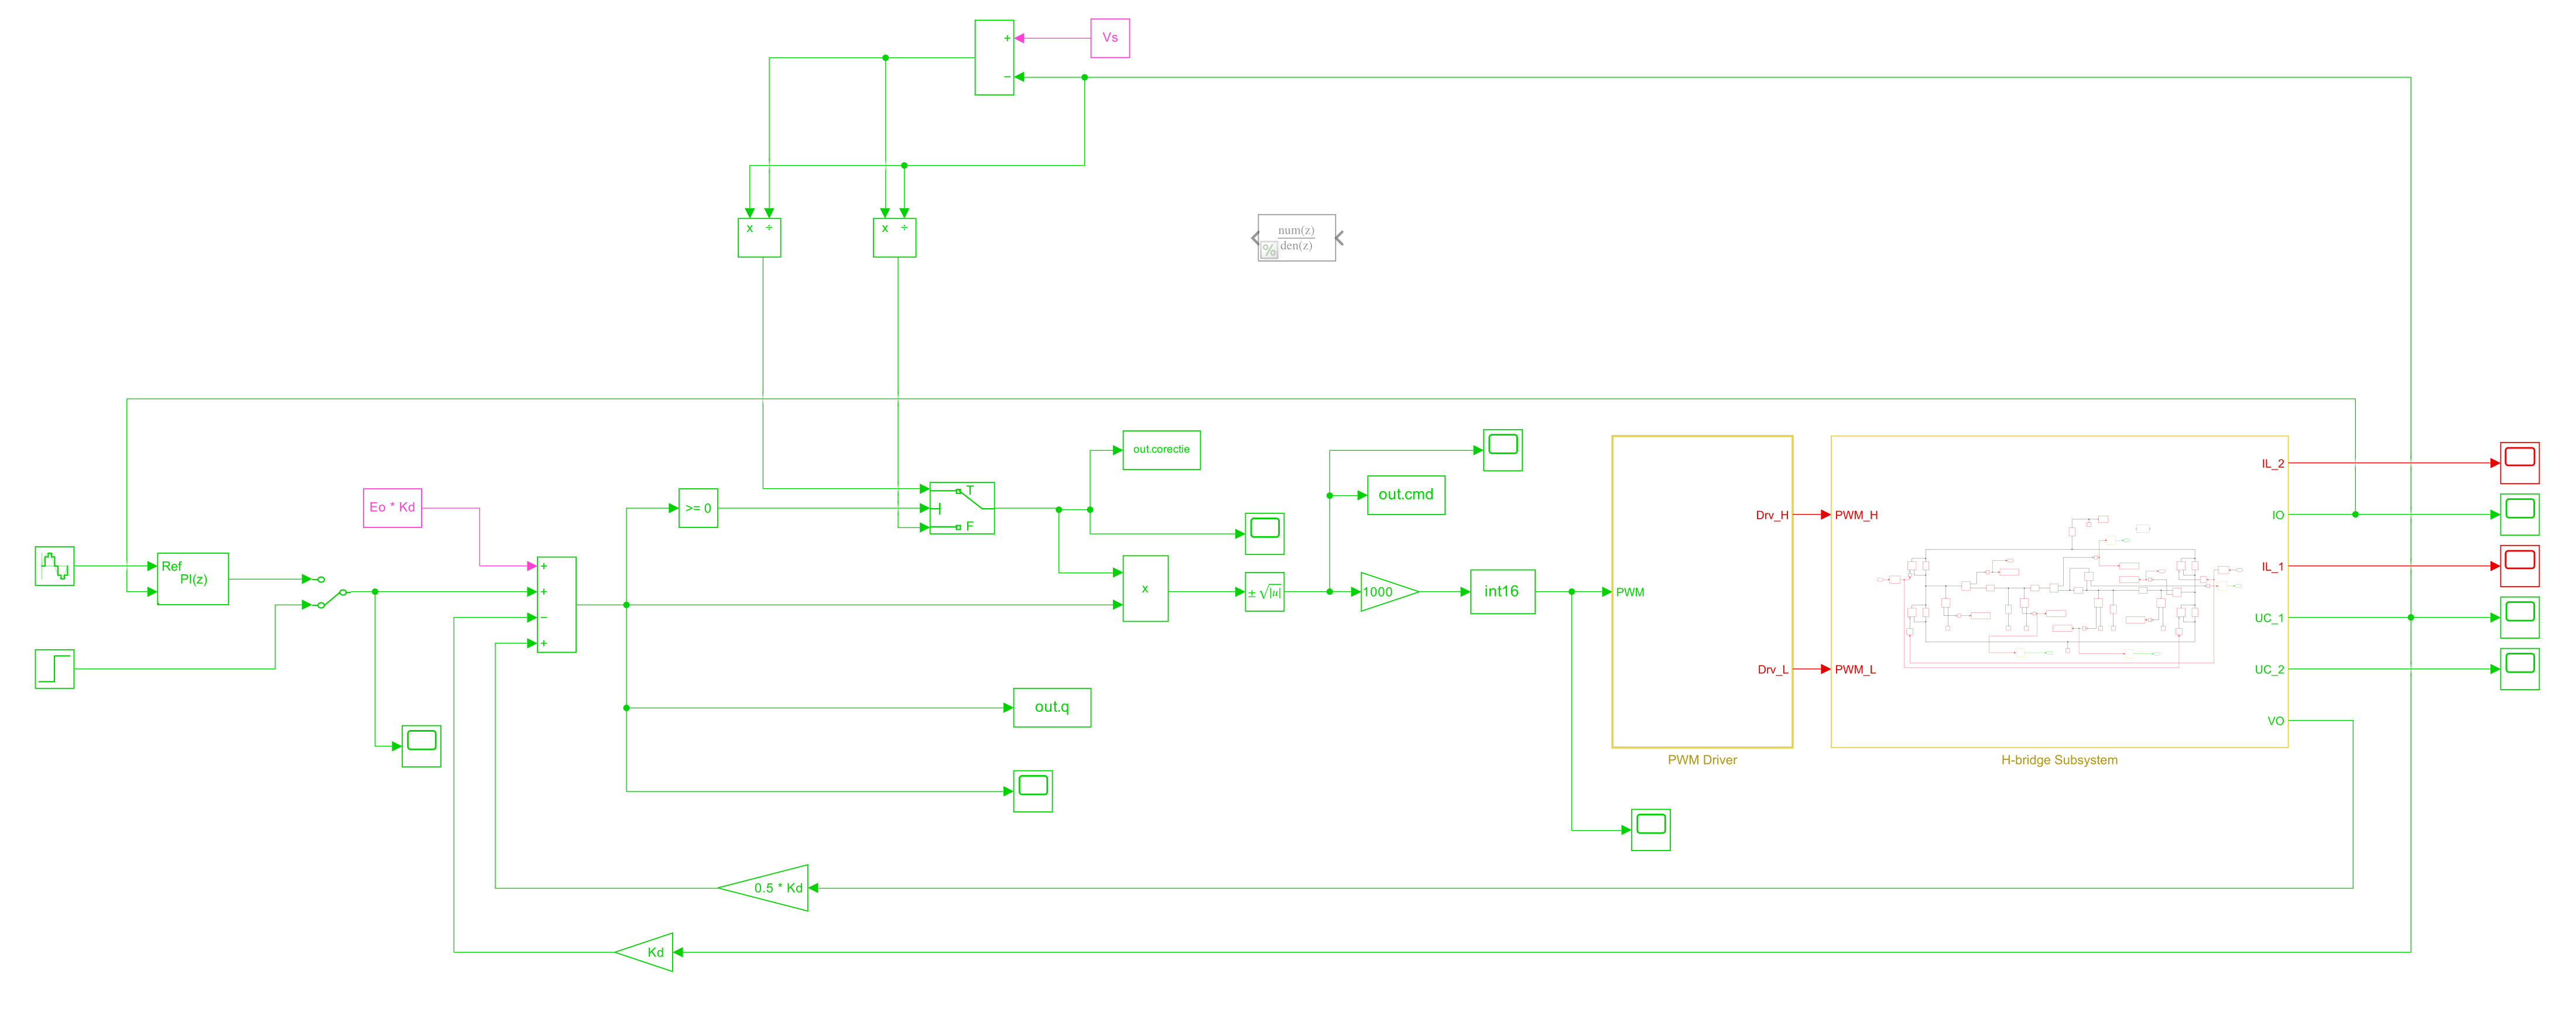
\includegraphics[width=0.92\paperwidth]{\pics/simulink/discuinv}
    }
    \caption{Complete Simulink Model, including control logic}
    \label{fig:discuinv}
\end{figure}

Besides the \gls{H-bridge} subsystem which as been presented previously, there is a \gls{pwm} generator block, which will be explained later in this section, and the feedback loop command subsection that is structured similar to the demonstrations given in \secref{sec:dcmctrl}.
When looking at equations \eqref{eq:newcmd} and \eqref{eq:timecalc}, the Simulink model adds a few more elements when compensating the effects of the output grid voltage that acts as a disturbance to the system.
The command generated has the formula:
\begin{equation}
    \begin{split}
        q(t) = E_o \cdot K_d + r(t) - I_o(t) \cdot h_r(t) - U_C(t) \cdot K_d + \frac{K_d}{2} \cdot V_o(t)
    \end{split}
\end{equation}
where $V_o$ is the output voltage of the converter and $h_r(t)$ is the inverse Laplace transform of the transform function for the \gls{pi} controller, where in the case of an open loop system, it does not exist.
To find the $K_p$ coefficient, we can stimulate the system with a step reference and see if there is a linear dependence between it and the stationary output of the system.
The graph that represents this can be seen in \figref{fig:openstepresp}
\begin{figure}[!ht]
    \begin{center}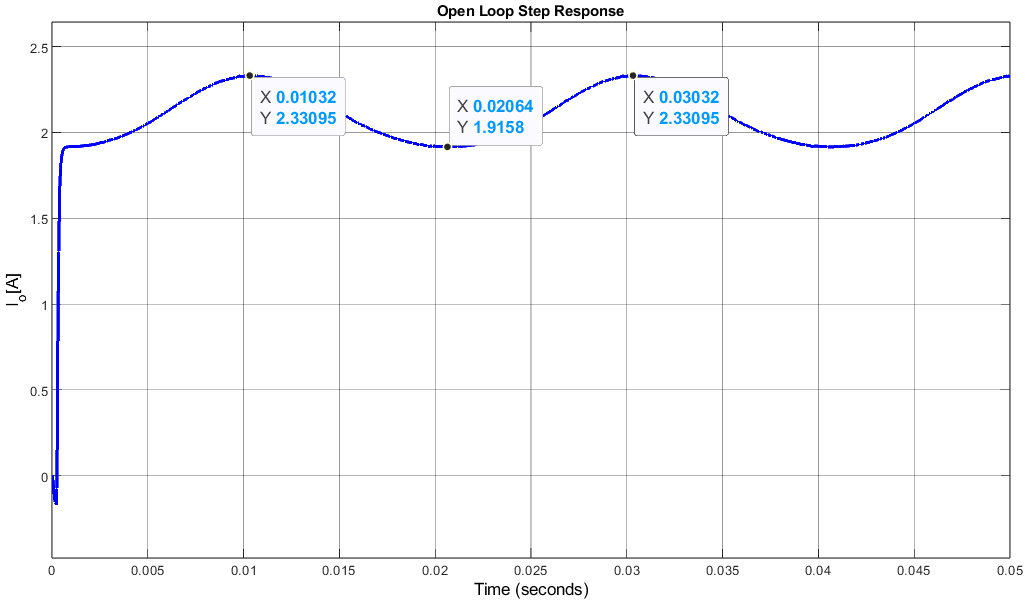
\includegraphics[width=\singlelongfigure]{\pics/simulink/openstepresp}\end{center}
    \caption{Step response of the open loop system}
    \label{fig:openstepresp}
\end{figure}

By giving multiple reference values, we can observe that output values follow a trend which can be seen in \tabref{tab:stepvals}.
\begin{table}[ht!]
\begin{center}
\begin{tabular}{|c|c|c|c|}
\hline
Step reference&Maximum stationary $[V]$&Minimum stationary $[V]$&Gain \\
value&sine value&sine value& \\ \hline
$0.1$&$2.33$&$1.92$&$21.25$ \\ \hline
$0.05$&$1.3$&$0.902$&$22.02$ \\ \hline
$0.15$&$3.33$&$2.89$&$20.73$ \\ \hline
$0.08$&$1.92$&$1.51$&$21.44$ \\ \hline
\end{tabular}
\end{center}
\caption{Step responses and respective gains}
\label{tab:stepvals}
\end{table}
If we are to assume the gain does not vary drastically from these points, we can choose any base $K_p \in [20, 22]$ that will approximate close to the real open loop system gain.
Now that $K_p \simeq 21$, $P \simeq 0.0119$, and by this, computing the integral term would result:
\begin{equation}
    I = \frac{P}{T} = \frac{P}{\sqrt{L_o C}} = 114.507
\end{equation}
With both controller coefficients found, we can replace them in the Simulink model and see the results of a sine wave response, which would be used in the real scenario of generating the \gls{ac} constant power source.
When running an experiment, the desired result should closely follow the reference signal provided, which for the one shown in \figref{fig:regcurrent}, the peak amplitude is chosen as $2.5A$ with the nominal frequency of $50Hz$ and no phase lag.
\begin{figure}[!ht]
    \begin{center}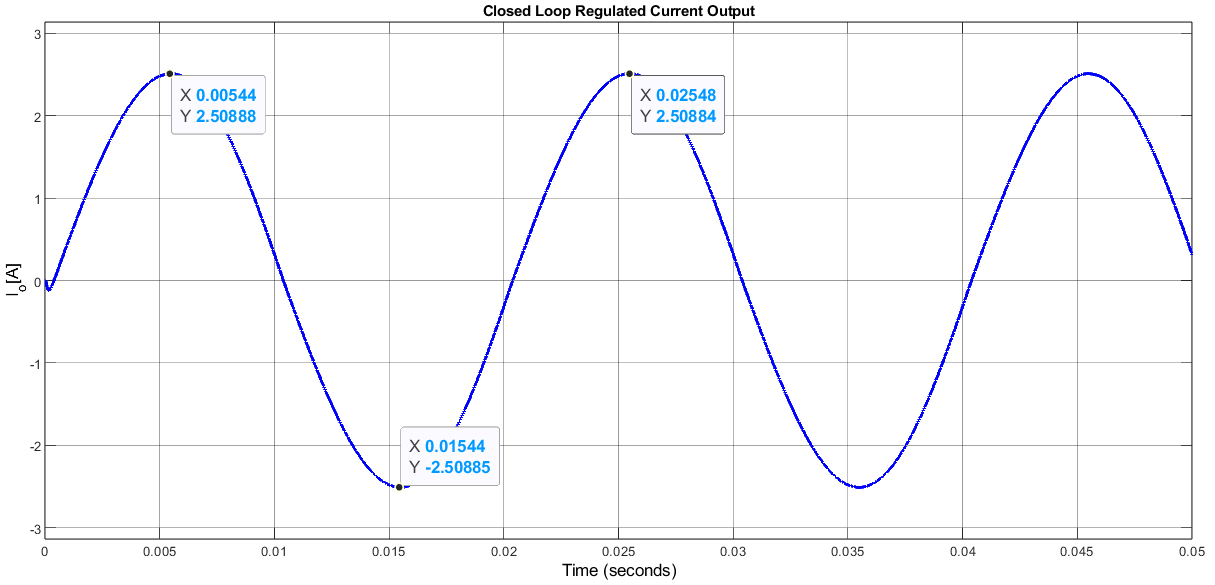
\includegraphics[width=\singlelongfigure]{\pics/simulink/regcurrent}\end{center}
    \caption{Regulated output current with sine wave reference}
    \label{fig:regcurrent}
\end{figure}
When testing, the regulator achieved the targeted value with a $\pm 10mA$ margin and retained the nominal frequency, however there is a noticeable undershoot at the beginning of the simulation of $400\mu s$, which stems from the unavoidable signal lag caused by the controller.
Other than that, the inductor current values and capacitor voltages do confirm the theoretical model proven in the \secref{sec:dcmctrl}.
\begin{figure}[!ht]
    \noindent
    \hspace*{-3.05cm}% Move left into the margin
    \begin{minipage}{\paperwidth}
        \subfloat[Current of the filter's inductors]{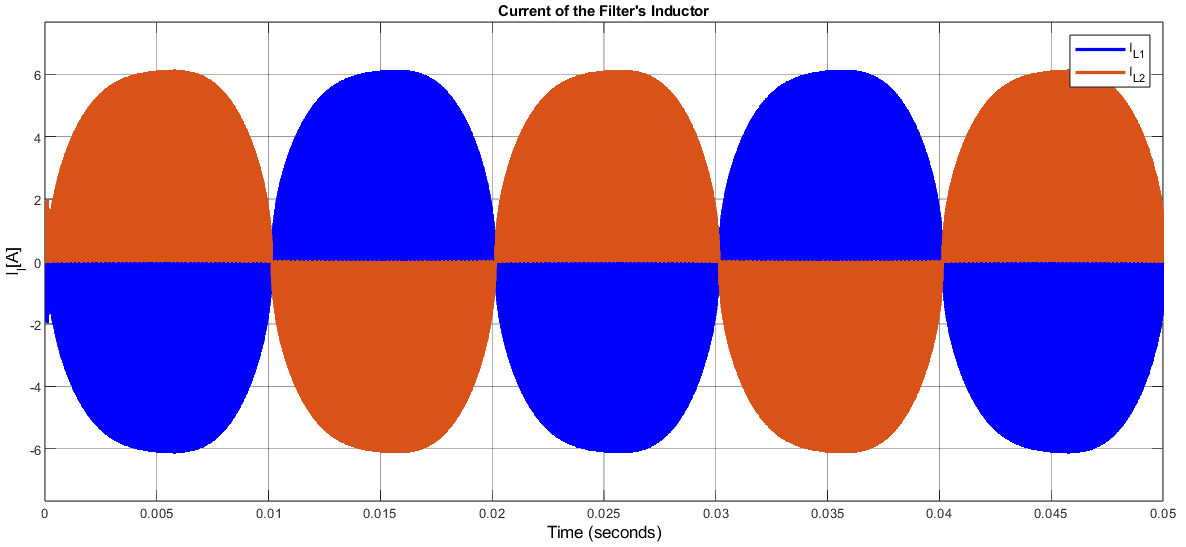
\includegraphics[width=0.5\paperwidth]{pics/simulink/indcur}}
        \hspace{0.01em}
        \subfloat[Voltage of the filter's capacitors]{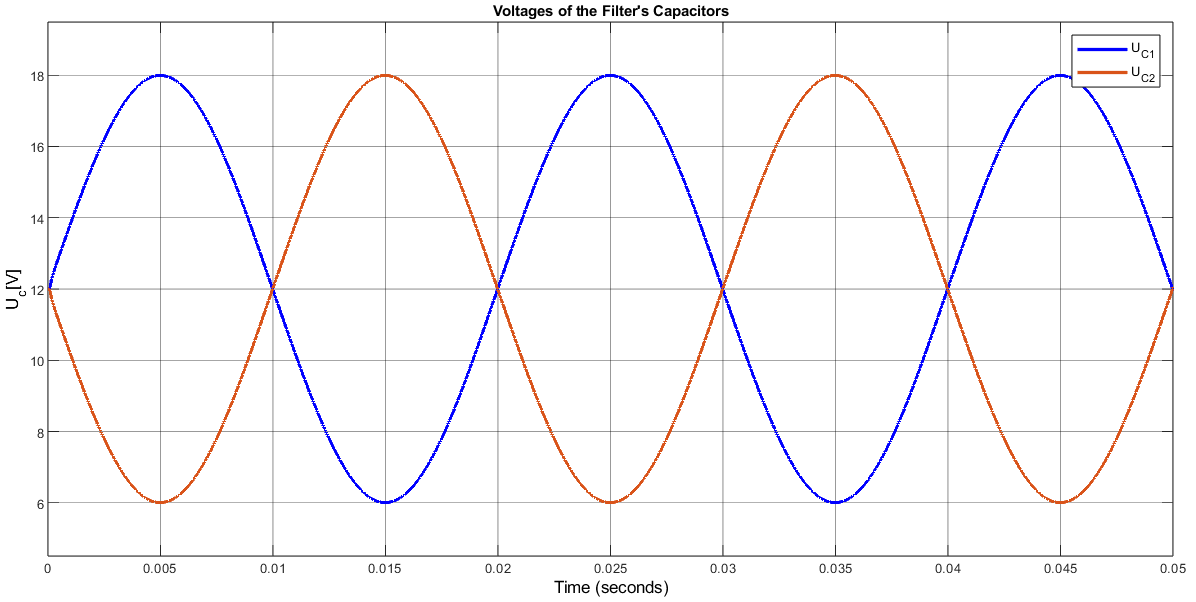
\includegraphics[width=0.5\paperwidth]{pics/simulink/capvolt}}
        \\[1em]
        \subfloat[PWM duty cycle value]{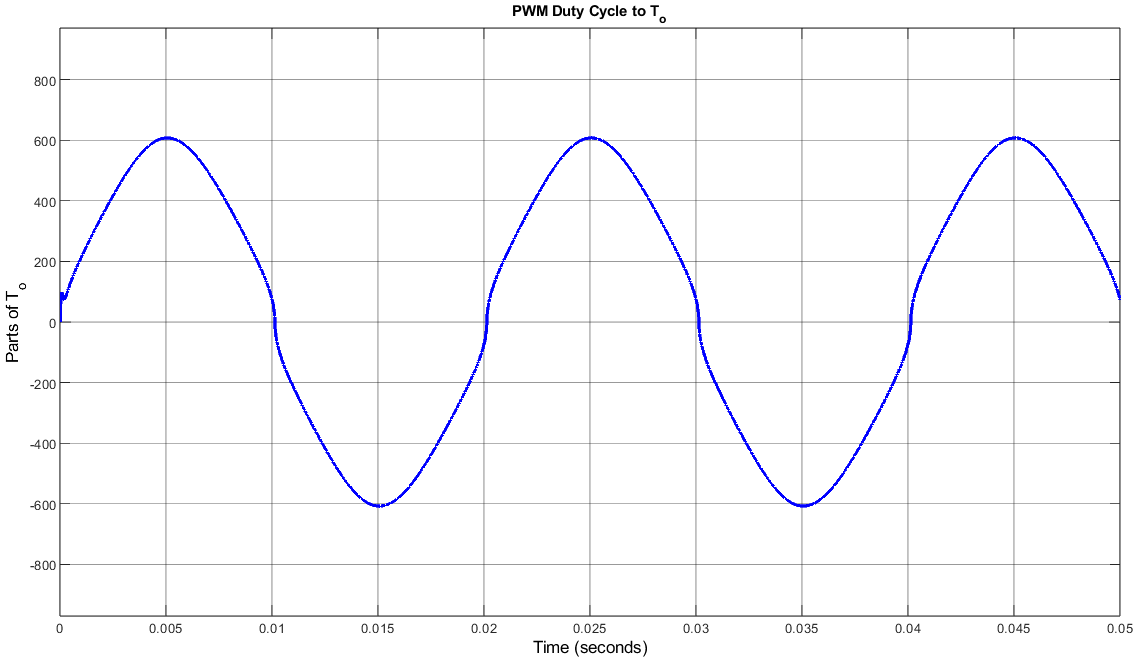
\includegraphics[width=0.5\paperwidth]{pics/simulink/pwmcyc}}
        \hspace{0.01em}
        \subfloat[Linearized and controlled command]{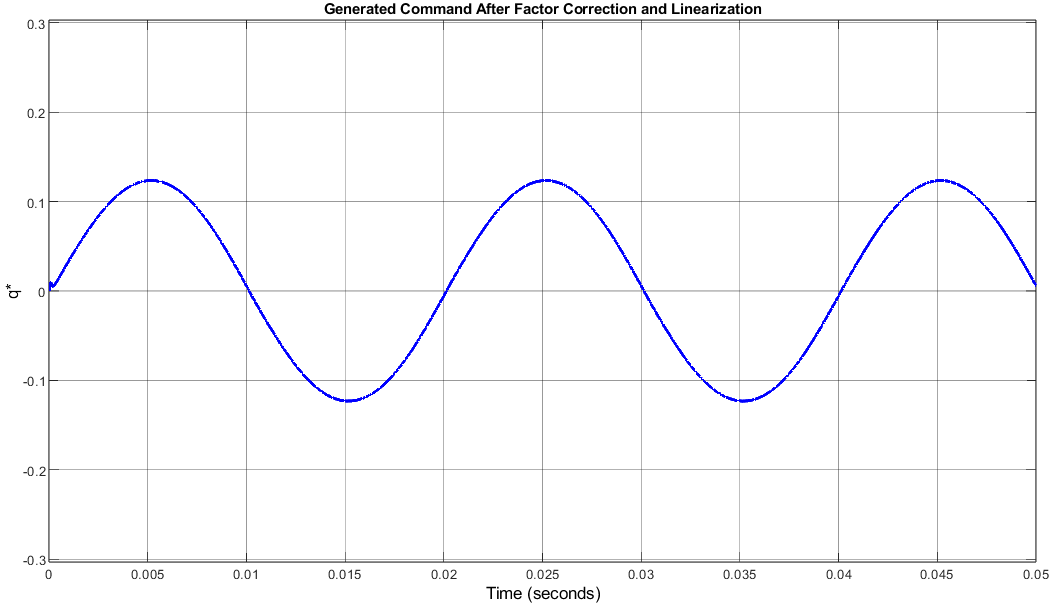
\includegraphics[width=0.5\paperwidth]{pics/simulink/gencmd}}
    \end{minipage}
    \caption{Circuit values from the successful test}
    \label{fig:simres}
\end{figure}
\begin{figure}[!ht]
    \noindent
    \hspace*{-3.05cm}% Move left into the margin
    \begin{minipage}{\paperwidth}
        \subfloat[Current of the filter's inductors, CCM section]{\label{fig:failsima}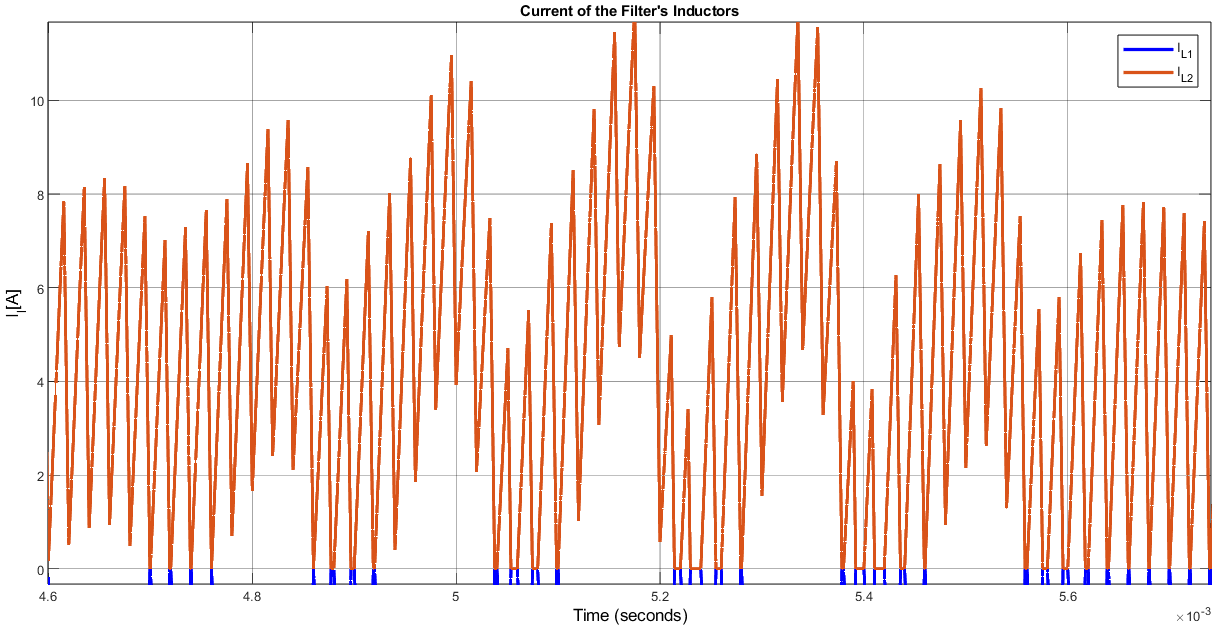
\includegraphics[width=0.5\paperwidth]{\pics/simulink/failindcur}}
        \hspace{0.01em}
        \subfloat[Regulated output current of the circuit]{\label{fig:failsimb}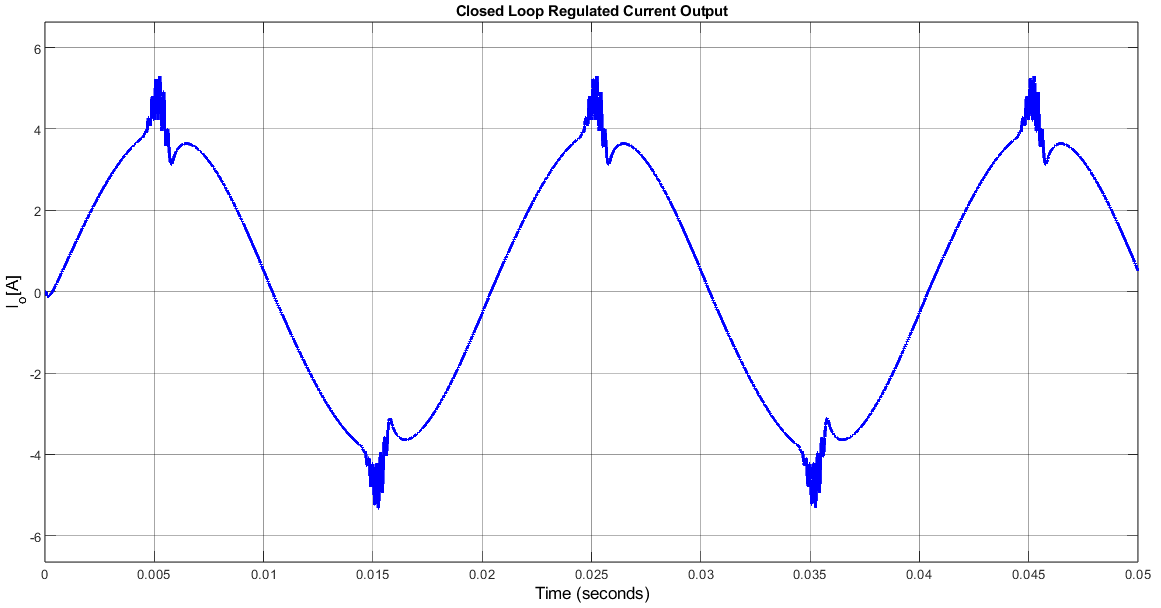
\includegraphics[width=0.5\paperwidth]{\pics/simulink/failregcurrent}}
    \end{minipage}
    \caption{Circuit values from the failed test}
    \label{fig:failsim}
\end{figure}
While the performances of the controller are, at a first glance, adequate, increasing the reference value of the controlled current to $4A$ results in an erroneous functioning of the controller.
This effect appears because the passive component filter is designed for certain operating conditions and by looking at \figref{fig:failsima}, the system enters \gls{ccm} as the inductor's current value has points at which it never drops to 0, meaning the system does not behave as expected of the controller.
This would mean that the designed \gls{pi} controller is performant for a specific target, but is not robust enough for higher outputs unless capacitance and inductance values are changed in accordance to the desired input and output power targets for the current conversion.

\begin{figure}[!ht]
    \centering
    \makebox[0pt]{
        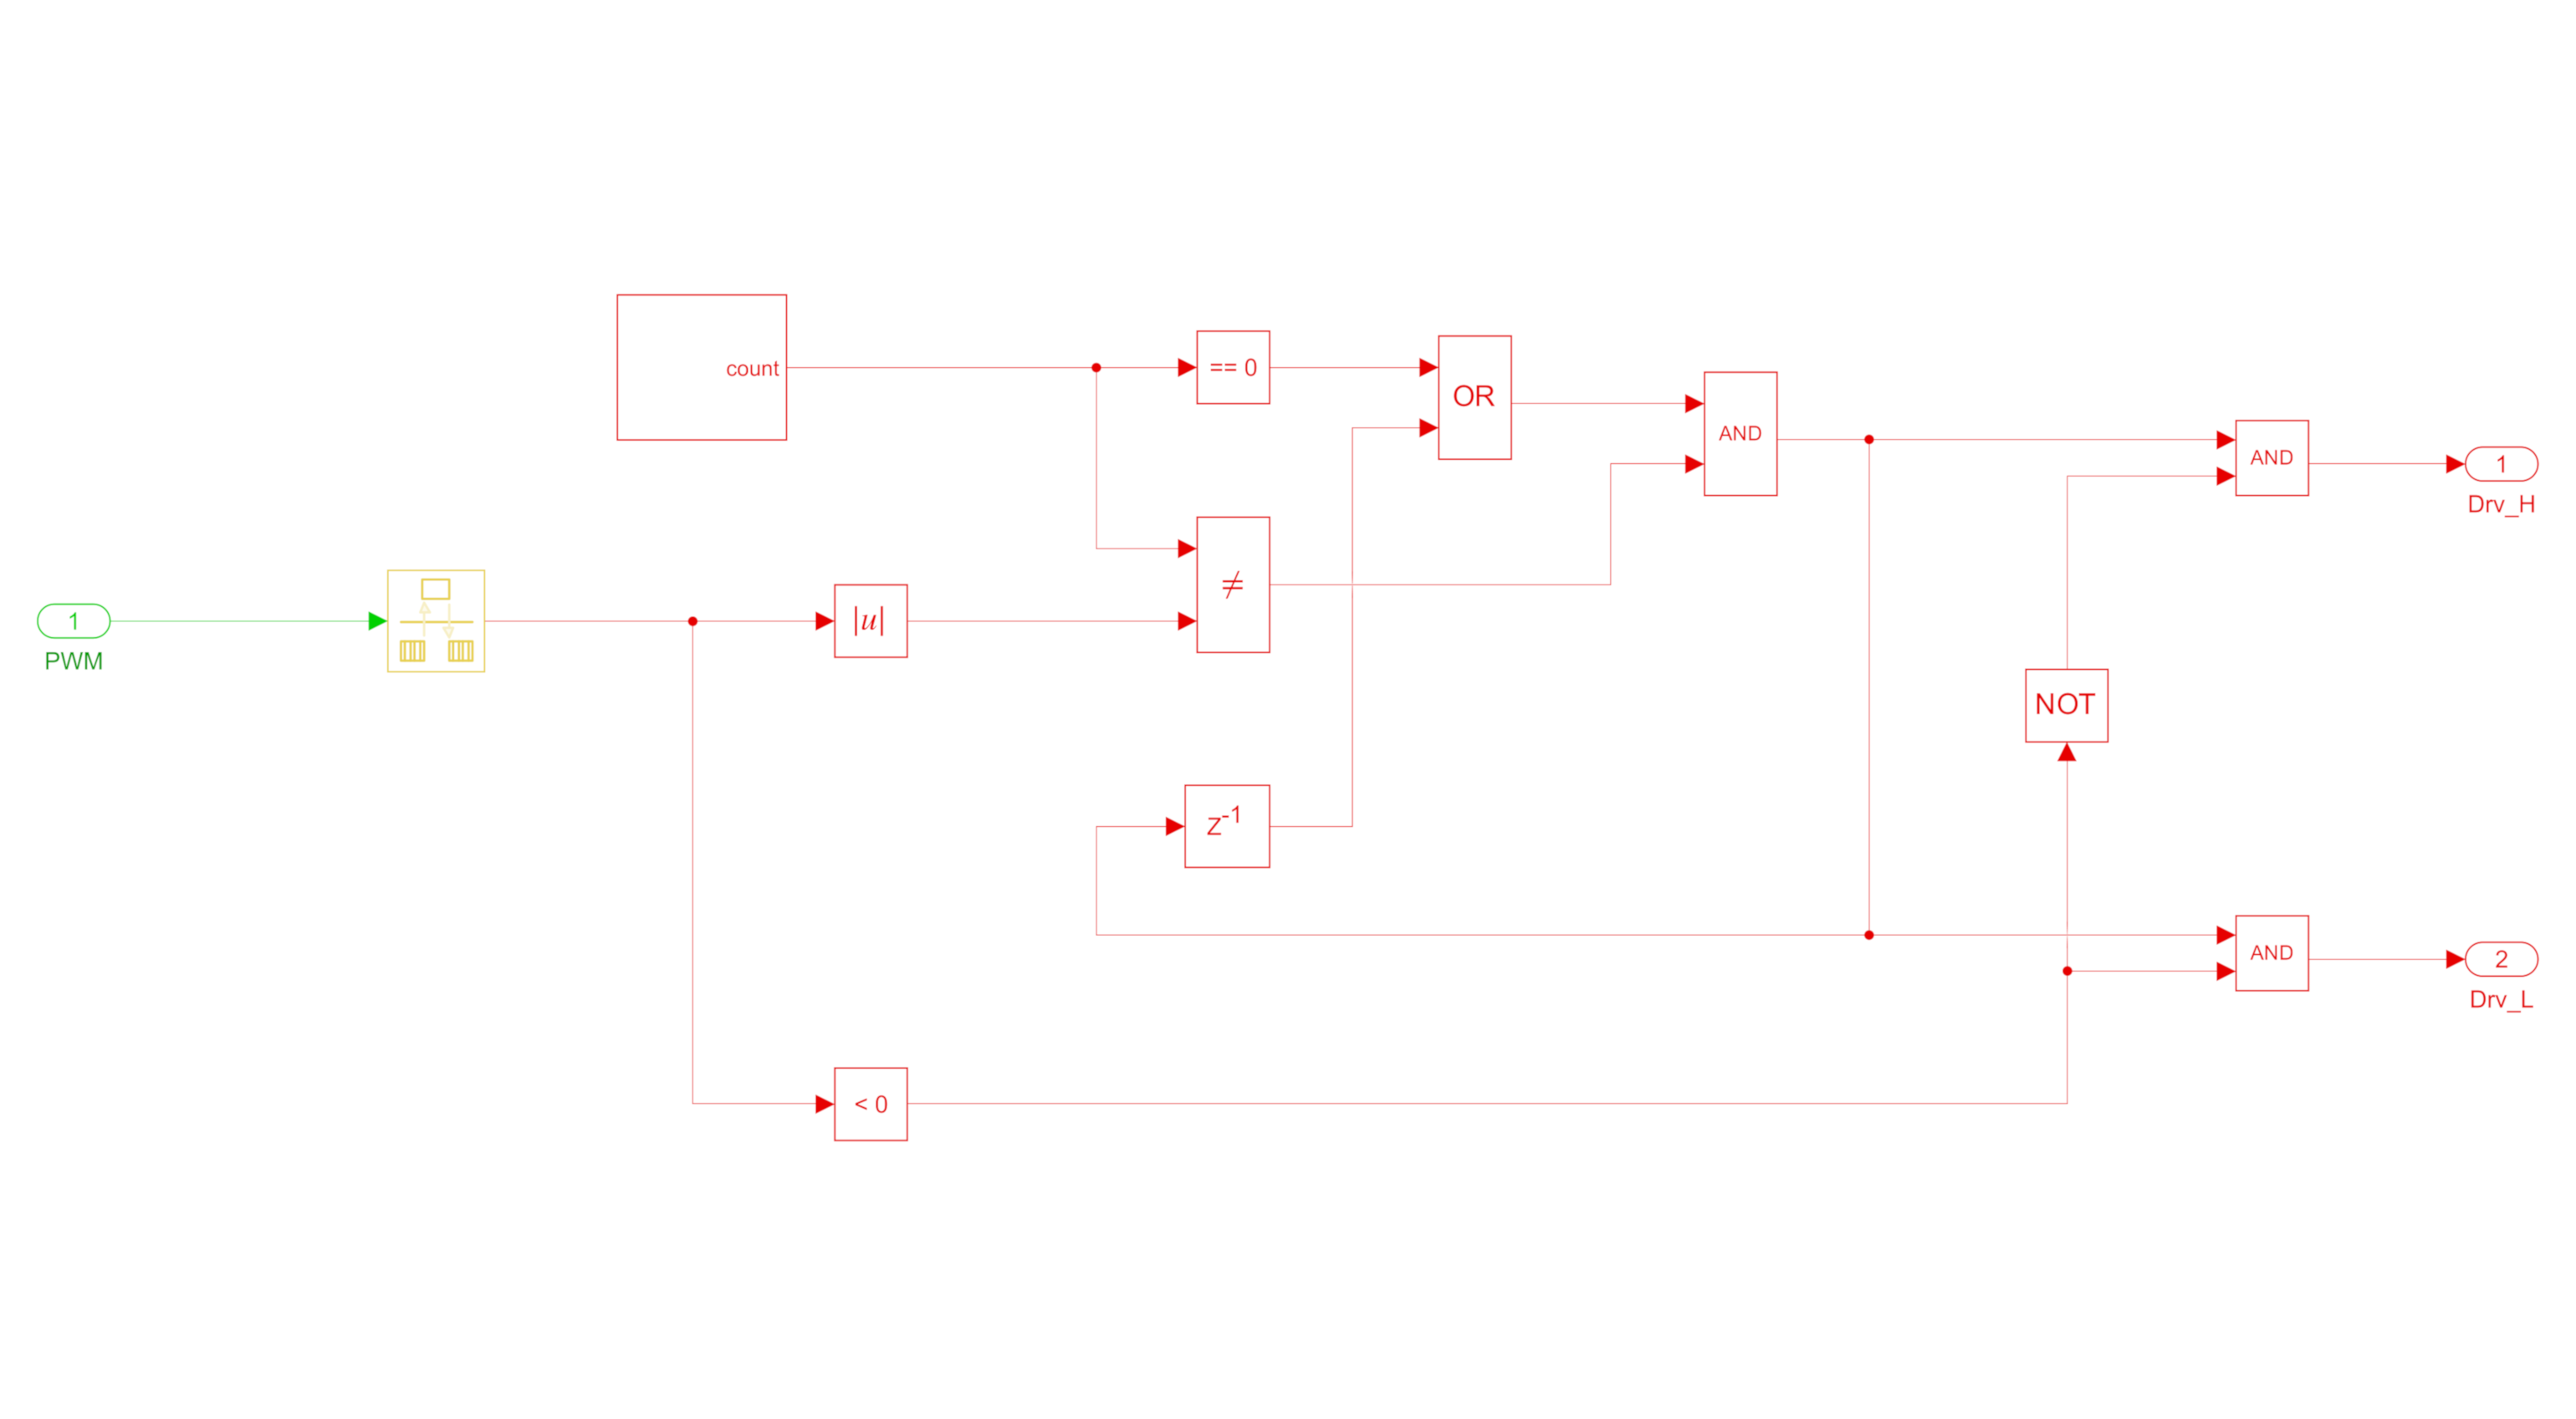
\includegraphics[width=0.90\paperwidth]{\pics/simulink/pwmdriver}
    }
    \caption{Simulink model of the PWM driver block}
    \label{fig:pwmdriver}
\end{figure}
The last remaining component of the system is the \gls{pwm} signal generator block, which converts the command value given by the feedback loop and creates the appropriate length of the duty cycle in relation to the available \gls{pwm} resolution.
The resolution is the ratio between the simulation sample time $T_s$ and the chosen \gls{pwm} time period of $T_o$, which result in $1000$ values, meaning a 10-bit resolution.
For the intent and purposes of this simulation, this bit depth satisfies minimal testing conditions, however this may be insufficient in real scenarios where a finer control is needed.
This is of course adjusted and given based on the capabilities of the hardware (specifically the microcontroller) chosen, where \gls{pwm} generator peripheral should function at the highest frequency available, since it is not indicated to change the time period of the associated \gls{pwm} signal as it also does change the behaviour of the linearization of the input command.
The command value represents $T_h$/$T_l$ compared to the bit-depth of the counter responsible for incrementing to $T_o$, and it is translated to the amount of time given to either the high/low-side transistor to be open, or switching from state $S_1$ to $S_2$.
This is done by creating a logic function which toggles the binary state when counting, setting it to high from the beginning until it reaches the command value, where it resets to low.
A simplified form is achieved using a Karnaught map for optimizing the logic function, as seen in \figref{fig:karnaught}.
\begin{figure}[!ht]
    \begin{center}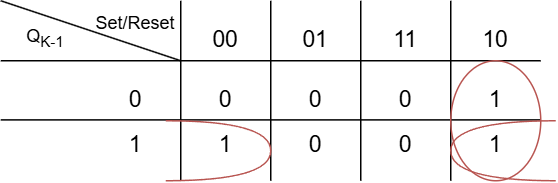
\includegraphics[width=\singlefigure]{\pics/simulink/karnaught}\end{center}
    \caption{Karnaught diagram of the logic function}
    \label{fig:karnaught}
\end{figure}
When writing the boolean equation, this would be the final result:
\begin{equation}
    \begin{split}
        Q_K &= S \cdot \overline{R} + Q_{K-1} \cdot \overline{R} \\
        &= \overline{R} \cdot (S + Q_{K-1})
    \end{split}
\end{equation}
Finally, only one side is active at a time, and to differentiate high-side from low-side the sign of the command is given as an argument to the output of each side, where positive means high and negative means low.